\documentclass[a4paper,14pt]{extreport}
  \usepackage[left=1.5cm,right=1.5cm,
      top=1.5cm,bottom=2cm,bindingoffset=0cm]{geometry}
  \usepackage{scrextend}
  \usepackage[T1,T2A]{fontenc}
  \usepackage[utf8]{inputenc}
  \usepackage[english,russian,ukrainian]{babel}
  \usepackage{tabularx}
  \linespread{1.3}
  \usepackage[colorinlistoftodos]{todonotes}
  \usepackage{amssymb}
  \usepackage{color}
  \usepackage{amsmath}
  \usepackage{mathrsfs}
  \usepackage{listings}
  \usepackage{graphicx}
  \graphicspath{ {./images/} }
  \usepackage{lipsum}
  \usepackage{xcolor}
  \usepackage{hyperref}
  \usepackage{tcolorbox}

  \usepackage[framemethod=TikZ]{mdframed}
  \usepackage{wrapfig,boxedminipage,lipsum}
  \mdfdefinestyle{MyFrame}{%
  linecolor=blue,outerlinewidth=2pt,roundcorner=20pt,innertopmargin=\baselineskip,innerbottommargin=\baselineskip,innerrightmargin=20pt,innerleftmargin=20pt,backgroundcolor=gray!50!white}
   \usepackage{csvsimple}
   \usepackage{supertabular}
  \usepackage{pdflscape}
  \usepackage{fancyvrb}
  %\usepackage{comment}
  \usepackage{array,tabularx}
  \usepackage{colortbl}

  \usepackage{varwidth}
  \tcbuselibrary{skins}
  \usepackage{fancybox}
  \usepackage{spreadtab}


  \usepackage{tikz}
  \usepackage[framemethod=TikZ]{mdframed}
  \usepackage{xcolor}
  \usetikzlibrary{calc}
  \makeatletter
  \newlength{\mylength}
  \xdef\CircleFactor{1.1}
  \setlength\mylength{\dimexpr\f@size pt}
  \newsavebox{\mybox}
  \newcommand*\circled[2][draw=blue]{\savebox\mybox{\vbox{\vphantom{WL1/}#1}}\setlength\mylength{\dimexpr\CircleFactor\dimexpr\ht\mybox+\dp\mybox\relax\relax}\tikzset{mystyle/.style={circle,#1,minimum height={\mylength}}}
  \tikz[baseline=(char.base)]
  \node[mystyle] (char) {#2};}
  \makeatother
   % Цвета для гиперссылок
  \definecolor{linkcolor}{rgb}{0, 0.72, 0.92} % цвет ссылок
  \definecolor{urlcolor}{rgb}{0.0, 0.0, 1.0}% цвет гиперссылок
  \hypersetup{pdfstartview=FitH,  linkcolor=linkcolor,urlcolor=urlcolor,citecolor=red, colorlinks=true}

  \definecolor{ggreen}{rgb}{0.4,1,0}
  \definecolor{rred}{rgb}{1,0.1,0.1}
  \definecolor{amber}{rgb}{1.0, 0.75, 0.0}
  \definecolor{babyblue}{rgb}{0.54, 0.81, 0.94}
  \definecolor{amethyst}{rgb}{0.6, 0.4, 0.8}

  \usepackage{float}
  \usepackage{wrapfig}
  \usepackage{framed}
  %for nice Code{
  \lstdefinestyle{customc}{
    belowcaptionskip=1\baselineskip,
    breaklines=true,
    frame=L,
    xleftmargin=\parindent,
    language=C,
    showstringspaces=false,
    basicstyle=\small\ttfamily,
    keywordstyle=\bfseries\color{green!40!black},
    commentstyle=\itshape\color{purple!40!black},
    identifierstyle=\color{blue},
    stringstyle=\color{orange},
  }
  \lstset{escapechar=@,style=customc}
%}


\begin{document}
\renewcommand{\bibname}{Список використаної літератури}% -- переименуем название списка литературы


%указатель -- \cite{lit1}

\pagecolor{white}

%----------------------------------------1
\newtcbox{\xmybox}[1][red]{on line, arc=7pt,colback=#1!10!white,colframe=#1!50!black, before upper={\rule[-3pt]{0pt}{10pt}},boxrule=1pt, boxsep=0pt,left=6pt,right=6pt,top=2pt,bottom=2pt}

\begin{titlepage}
  \begin{center}
  \large
  Національний технічний університет України \\ "Київський політехнічний інститут імені Ігоря Сікорського"


  Факультет Електроніки

  Кафедра мікроелектроніки
  \vfill

  \textsc{РЕФЕРАТ}\\

  %{\Large Про виконання лабораторної роботи №1\\
  з дисципліни: «Функціональна електроніка»\\[1cm]

  Шляхи збільшення густини запису інформації при магнітному записі


  %}
  \bigskip
  \end{center}
  \vfill

  \newlength{\ML}
  \settowidth{\ML}{«\underline{\hspace{0.4cm}}» \underline{\hspace{2cm}}}
  \hfill
  \begin{minipage}{1\textwidth}
  Виконавець:\\
  Студент 4-го курсу \hspace{4cm} $\underset{\text{(підпис)}}{\underline{\hspace{0.2\textwidth}}}$  \hspace{1cm}Мнацаканов А. С.\\
  \vspace{1cm}

  Перевірила: \hspace{5.6cm} $\underset{\text{(підпис)}}{\underline{\hspace{0.2\textwidth}}}$  \hspace{1cm}  Обухова Т. Ю.\\

  \end{minipage}

  \vfill

  \begin{center}
  2021
  \end{center}
\end{titlepage}
\tableofcontents
\setcounter{page}{2}

\newpage

\chapter{Відкриття та розвиток магнітного запису}\par
  %\section{Подраздел}

  Перший апарат магнітного запису винайшов і побудував датський інженер Вальдемар Поульсен. Апарат назвали телеграфоном (\ref{ris2}) і призначався він для
  зберігання звуку. Телеграфон був запатентований в 1898 році\cite{lit1}, і цю дату вважають роком народження магнітного запису.\par
    \begin{figure}[h]
    \center{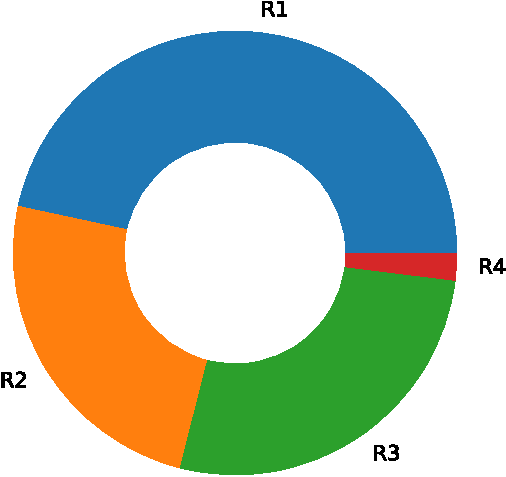
\includegraphics[width=0.7\linewidth]{2.jpg}}
    \caption{Перший апарат магнітного запису.}
    \label{ris2}
  \end{figure}
  Поульсен створив кілька різновидів апаратів для магнітного запису. В одному з них дріт (носій запису) намотаний на немагнітний валик, який утворює на ньому магнітний робочий шар у вигляді циліндричної спіралі. В процесі запису або відтворення валик разом з дротом
  обертався відносно магнітної головки, яка переміщалася паралельно його осі, ковзаючи по виткам дроту, як по різьбі гвинта. В ролі магнітної головки використовувався електромагніт, що складався з стрижневого осердя, який одним кінцем ковзав по носію, і
  котушки мідного дроту. Головка з сердечником створювала досить сильне і сконцентроване магнітне поле, за допомогою якого можна було записувати звукові частоти.\par

  У 1906 році в США був виданий перший патент на магнітний диск зі суцільним магнітним покриттям. В цей же період розвитку
  магнітного запису в якості носія застосовували також і сталеву катану стрічку\cite{lit1}. Дротові і стрічкові носії запису того часу мали досить низькі властивості. Однак носії з високими, за сучасними поняттями, властивостями, можливо, взагалі не дозволили б реалізувати в той час магнітний запис. Дріт і сталева стрічка мали низьку коерцитивну силу, високу залишкову індукцію і велику товщину, що давало
  змогу здійснювати магнітний запис і відтворення без посилення сигналів. Струм звукового сигналу безпосередньо від мікрофона і батареї
  надходив в головку, що намагнічує носій запису. Записати таким чином звуковий сигнал на сучасний висококоерцетивний носій дуже важко.\par
  
  У 1925 році І.І. Крейчману в СРСР і в 1928 році Ф. Пфлеймеру в Німеччині були видані патенти на носії запису, у яких на паперову,
  пластмасову або на будь-яку іншу гнучку немагнітну підкладку наносився робочий шар, що складався з магнітного порошку,
  диспергированного в немагнітної сполучною середовищі. Цей тип носія у вигляді порошкової магнітної стрічки надалі отримав найбільше
  поширення.\par

  У 1932 р \href{https://ru.wikipedia.org/wiki/%D0%91%D0%B8-%D0%B1%D0%B8-%D1%81%D0%B8}{BBC} вперше застосувала апарат магнітного запису на тонкій сталевій стрічці, шириною 3 мм і товщиною 0,08 мм. Швидкість руху стрічки щодо головок 1,5 м/с щодо записувальної та відтворювальної головок. На півгодинну програму йшло 3 км стрічки, а котушка з стрічкою важила 25 кг.\par
  \vspace{0.5cm}
   \begin{figure}[h]
    \center{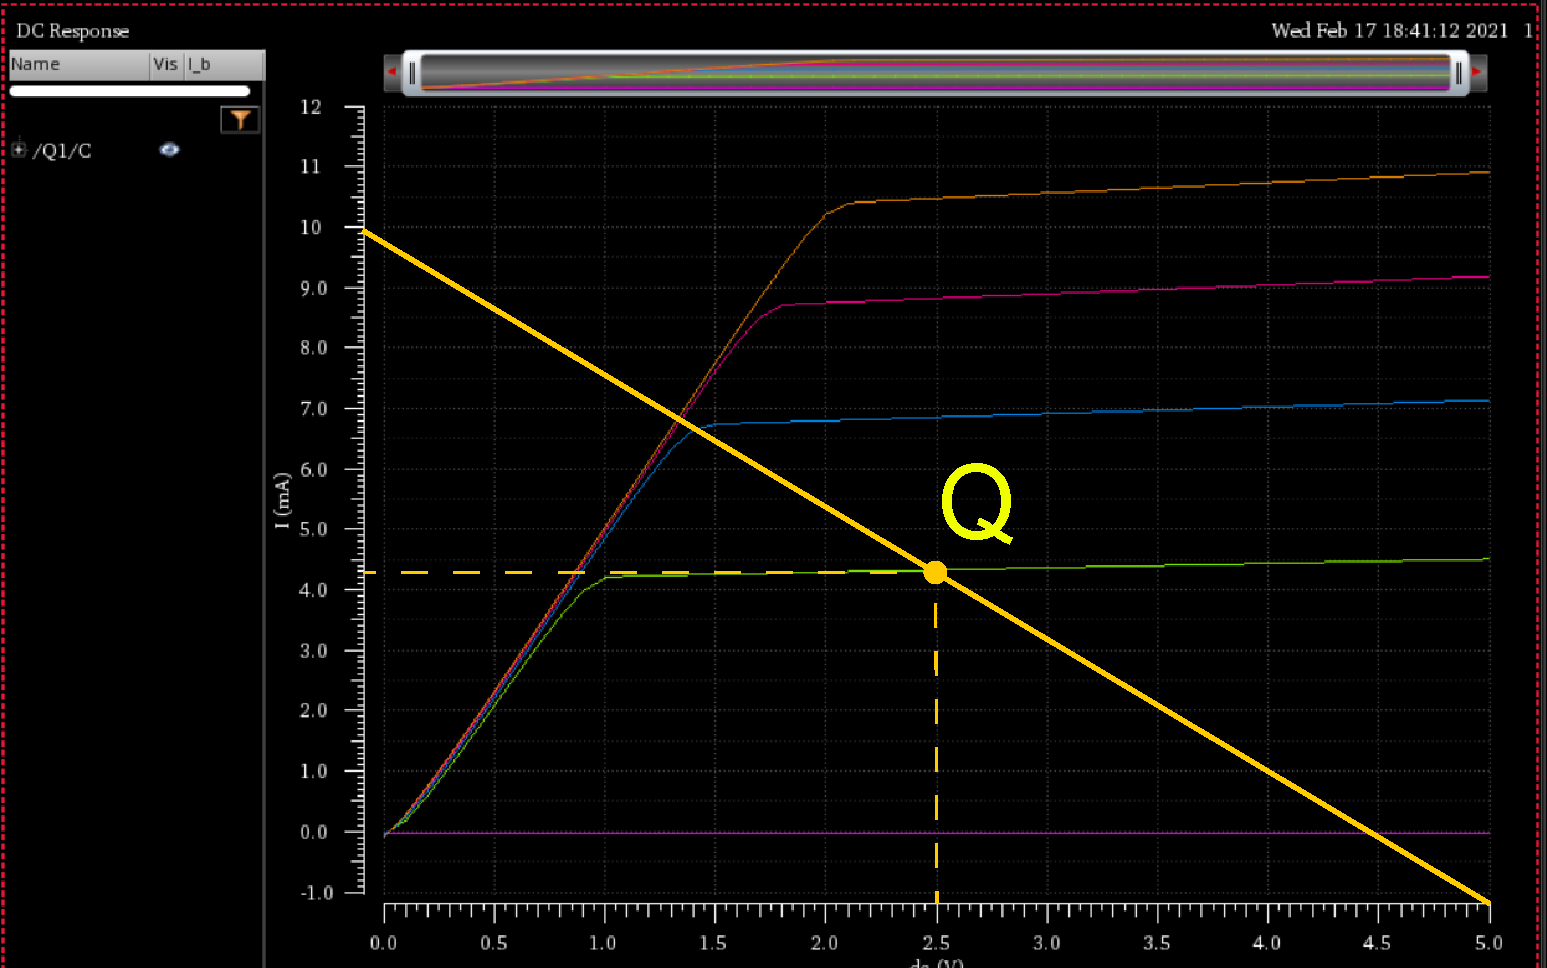
\includegraphics[width=0.75\linewidth]{1.png}}
    \caption{Структура шарів магнітної стрічки.}
    \label{ris1}
  \end{figure}

  У 1934 році фірма IG Farben в Німеччині випустила першу промислову партію магнітної стрічки, у якій на підкладку з
  ацетилцелюлози нанесено робочий шар, що містить порошок карбонільного заліза. У 1939 році ця ж фірма створила стрічку з більш стабільним і більш дешевим магнітним порошком гамма-оксиду заліза.\par

  До початку 40-х років 20 століття різні дослідники незалежно один від іншого встановили, що, якщо в головку запису поряд з струмом записуваного сигналу подавати струм високої частоти (в 5-6 разів вище частоти сигналу), сигнал буде записаний на носії з дуже малими спотвореннями.\par 

  50-ті роки - період особливо інтенсивного розвитку магнітного запису. В 1952 року почали використовувати магнітні стрічки для запам'ятовування інформації в ЕОМ, а в 1956 році для запису телевізійних передач.\par

  У 60-70 роки розвиток носіїв магнітного запису тривав як в
  напрямку розробки нових матеріалів, так і в розширенні асортименту
  носіїв. Був створений новий магнітний порошок, що складається з діоксиду хрому, з високими магнітними властивостями. З'явилися нові модифікації порошків оксиду заліза з більш дрібними частинками і з добавкою кобальту. В кінці 70-х - початку 80-х років майже завершився цикл у розвитку носіїв магнітного запису на стрічки оскільки цей вид запису програє у швидкості самого запису та зчитуванні з носія інформації.

\chapter{Структура пристроїв запису(зчитування)}\par
  Узагальнену структурну схему апаратури точного магнітного запису -- АМЗ, можна представити у вигляді, наведеному на рис. \ref{ris3}.
  На ньому виділені такі складові частини, як електронний блок запису 1, механізм протягування стрічки 2 і електронний блок відтворення 3. Блок записи 1 включає в себе вхідні перетворювачі 4, модуляційні пристрою 5, підсилювачі запису 6 і генератор опорного
  або контрольного пілот-сигналу 7. Стрічкопротяжний механізм 2 містить магнітні головки запису 8 і відтворення (зчитування) 11
  (Або універсальні магнітні головки), приймальню і подає касети 9 і магнітний носій 10. Блок відтворення складається з підсилювачів відтворення (зчитування) 12, демодуляторів 13, вихідних
  перетворювачів 14, детектора временнóй помилки 15 і блоку регулювання (компенсації часової помилки) 16.\par

  Слід зазначити аналогію між наведеною узагальненою структурною схемою АМЗ і блок-схемою каналу зв'язку, що складається з передавача 1, середовища поширення сигналів, що передаються 2 і приймача 3.
  В цьому випадку блоки 7, 15 і 16 грають роль синхронізуючих пристроїв. Така аналогія обумовлена тим, що і канал зв'язку, і АМЗ призначені для передачі електричних сигналів: перший - в просторі, другий - в часі.\par

  Великий парк різноманітних типів експлуатованої і знову розробляється АМЗ можна класифікувати за різними ознаками:
  \begin{itemize}
    \item по виду використовуваної модуляції сигналу;
    \item за обсягом інформації, що запам'ятовується, який залежить від числа
    каналів (або доріжок на магнітному носії), їх смуги пропускання,
    швидкості протягання і довжини носія (т. е. час запису сигналу) і
    амплітудного діапазону реєстрованого електричної напруги);
    \item по можливій послідовності застосування режимів запісі-
    відтворення (наприклад - режим тільки записи на борту і режим
    тільки відтворення при приземленні літального апарату, режим
    одночасного запису і відтворення з фіксованою затримкою
    відтвореного сигналу щодо записується і т. д.);
    \item щодо забезпечення можливості транспонування швидкості руху
    носія в режимі відтворення, що призводить до трансформації
    спектра записаного сигналу;
    \item за типом застосованого магнітного носія (магнітна або металева стрічка, дріт, барабан, диск);
    \item за призначенням, умовами експлуатації і особливостям конструкції (бортова або наземна апаратура, форма тракту стрічкопротяжного
    механізму: відкритий, закритий U-образний, замкнуте кільце; котушкові або компакт-касети і т. д.);
    \item по масо-габаритних характеристиках, енергоспоживанню, і ін.
  \end{itemize}

    \begin{figure}[h]
      \center{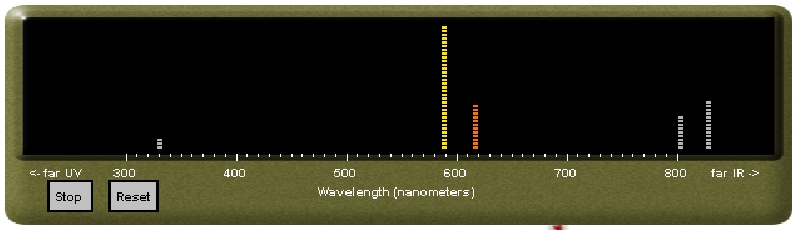
\includegraphics[width=0.75\linewidth]{3.png}}
        \caption{Узагальнена структурна схема апаратури точного магнітного запису.\\ 1 - електронний блок запису; 2 - механізм протягування стрічки;
        3 - електронний блок відтворення; 4 - вхідний перетворювач;
        5 - модулятор; 6 - підсилювач запису; 7 - генератор пілот-сигналу;      8 - магнітна головка запису; 9 - касета; 10 - магнітний носій;      11 - магнітна головка відтворення; 12 - підсилювач відтворення;      13 - демодулятор; 14 - вихідний перетворювач; 15 - детектор часової помилки; 16 - блок регулювання; $U_{i_{\text{вих}}}$ - вхідний реєстрований сигнал; $U_{i_{\text{вих}}}$ - вихідний електричний сигнал}
      \label{ris3}
    \end{figure}

\chapter{Основні джерела спотворень сигналів вимірювальної інформації в каналах магнітного запису-відтворення}\par

  Дослідженню причин спотворень сигналу в каналі магнітного запису-відтворення присвячена велика кількість робіт вітчизняних і
  зарубіжних авторів.
  Як було досі виявлено основними причинами спотворень сигналу є:
  \begin{itemize}
  \item частотні спотворення, що виникають в системі магнітна головка-
  стрічка-головка і в електронних блоках запису-відтворення;
  \item фазові спотворення, що виникають в електронних блоках записи -
  відтворення і в системі головка-магнітна стрічка-головка;
  \item нелінійність амплітудних характеристик електронних блоків і
  процесу запису сигналу в системі головка-стрічка;
  \item  паразитна амплітудна модуляція;
  \item шум стрічки;
  \item перехідні перешкоди;
  \item  ефект проникнення;
  \item копіювальний ефект;
  \item ефект саморозмагнічування;
  \item дефекти і пошкодження магнітного носія;
  \item шум електронних блоків запису і відтворення;
  \item коливання, дрейф і неномінальність швидкості руху магнітної стрічки;
  \item статичний і динамічний перекоси магнітної стрічки щодо робочого зазору головки;
  \end{itemize}



\chapter{Сучасні носії информації}
Взагалі, багато інформації в світі зберігається саме на стрічці: наукові дані про фізику частинок, астрономічні дані, національні архіви, культурну спадщину, більшість кінофільмів, банківські дані і так далі. Існують професіонали (фахівці з матеріалами, інженери, фізики), чия робота - удосконалювати способи зберігання даних на плівці.\par

За останнє десятиліття плівка розвивалася не менш, ніж жорсткі диски або транзистори. Перша плівка для зберігання інформації в цифровому вигляді - модель 726 виробництва IBM - могла зберігати 1,1 МБ на котушці. Сьогодні 1 котушка здатна зберігати 15 терабайт даних, а одне роботизоване плівкове сховище - 278 петабайт.\par

Звичайно, плівка не дозволяє так само швидко зчитувати інформацію, як жорсткі диски або напівпровідникова пам'ять. Але у неї є свої переваги. Плівка енергоефективна: якщо дані вже записані, плівці не потрібно споживати електроенергію для їх зберігання. Плівка надійна: ймовірність помилок при записі або читанні на 4-5 порядків нижче, ніж у жорстких дисків. Плівка безпечна: на відміну від дисків, які, як правило, підключені до комп'ютера постійно, картриджі з котушками можуть зберігатися без підключення до пристроїв, що захищає дані на плівці від читання або модифікації зловмисниками або від помилок через людський фактор.\par

У 2011 році через помилку в ПО на серверах Google випадково видалив пошту в 40000 ящиках. Видалення відбулося на всіх резервних копіях на жорстких дисках, тому що помилкову операцію ланцюжком пройшла і по ним, але листи вдалося відновити з 
плівки. Після цього випадку вперше стало відомо, що Google робить  резервні копії на плівці, а потім і Microsoft підтвердили, що в їх хмарному сервісі Azure використовують плівкове обладнання IBM.\par

Зберігати дані на плівці в 6 разів дешевше, ніж на жорстких дисках, тому вона використовується повсюдно, якщо мова йде про великих обсягах інформації. Так як плівка практично зникла з споживчого ринку, більшість і не знає, як стрімко вона розвивається і буде розвиватися в найближчому майбутньому.\par

Плівка \textquotedblleft вижила\textquotedblright, оскільки вона мізерно дешева, і дешевшає з часом. Можна припустити, що, раз ущільнення запису даних на жорстких дисках сходить нанівець, то те ж саме можна застосувати і до плівки, тому що для неї використовується приблизно та ж технологія (тільки старіша). Це як «закон Мура», але для магнітної плівки. Але це не так: з роками темпи ущільнення записи на плівці не спадають, а зберігаються в районі 33\% в рік. Тобто, подвоєння обсягу даних, записаних на плівці, відбувається приблизно кожні 2-3 роки.

Фізично технологія запису на жорсткі диски і плівки одна і та ж: дані записуються на намагнічену поверхню вузькими доріжками, на яких відбувається перемикання полярності. Інформація записується послідовністю бітів. З моменту появи плівки і жорстких дисків в 50-х, виробники того і іншого прагнуть до більшої щільності, швидкості і дешевизні, тому вартість зберігання в доларах на гігабайт знизилася на порядки. Саме через те, що виробництво намагаються здешевити, росте щільність запису на квадратний міліметр.\par

Чим більше фінансування на дослідження і розробку отримують компанії, що виробляють магнітні носії, очевидно, тим більше ці носії прогресують. Зараз на найбільш просунутих жорстких дисках можна записати в 100 разів більше інформації, ніж на такій же площі плівки. Але так як самої цієї площі на плівці в котушці набагато більше, на ній поміщається до 15 ТБ даних, що більше, ніж на будь-яких існуючих на ринку дисках. При цьому габарити картриджа з котушкою плівки і жорсткого диска приблизно однакові.\par

Крім місткості у плівки і жорстких дисків є ще відмінність: швидкість доступу до даних. У котушках знаходяться магнітні стрічки довжиною в кілька сотень метрів, середній час доступу до даних - від 50 до 60 секунд. У жорстких дисків цей час - від 5 до 10 мілісекунд. Однак, швидкість запису на плівку при цьому вдвічі вище\cite{lit2}.\par

За останні роки темпи ущільнення запису на дисках зменшилися з 40\% до 15\% в рік. Причина - фундаментальна фізика. Щоб записати більше даних на колишньої площі, потрібно зменшити область для запису кожного біта. Як наслідок, це зменшує силу сигналу під час читання даних. Якщо занадто зменшити силу сигналу, то він може змішатися з магнітним шумом від сусідніх магнітних гранул, що покривають поверхню диска. Можна зменшити і шум, зробивши самі гранули менше. Але тоді гранула буде вже настільки мала, що навряд чи зможе стабільно утримувати свою намагніченість. Найменший розмір гранул, придатний для магнітного запису, вже досягнуто, в професійній області його називають супермагніченою межею\par.

До недавнього часу досягнення цієї межі залишалося для споживачів непомітним, тому що виробники додавали всередину контейнера додаткові диски та головки для запису і читання, роблячи жорсткий диск колишнього розміру, але більшого обсягу. Однак тепер і більше дисків всередину контейнера вже складно додати, зберігши його розміри, тому межа стає помітнішою.\par

Є альтернативні способи запису на магнітну поверхню, які теоретично можуть подолати супермагнетичну межа. Це запис, що супроводжується нагріванням гранул, і мікрохвильовий запис. Але це складно в інженерному та фінансовому аспекті. Компанія Western Digital анонсувала жорсткий диск з мікрохвильовим способом запису, який вона збиралась випустити в 2019 році. Очікувалось, що така інновація дозволить зберегти темпи ущільнення записи в районі 15\% в рік.\par

У той же час зберігання на плівці ще далеко від досягнення супермагнетичної межі, тому плівка десятиліттями може еволюціонувати, не спираючись на свій «закон Мура» і обмеження фундаментальної фізики.\par

У плівки хитра природа. Зміна картриджів з котушками в записуючому обладнанні, тонкий полімерний матеріал, паралельний запис на 32 доріжках - все це створює складності в дизайні цього носія інформації.\par

У 2015 році компанія IBM у співпраці з корпорацією FujiFilm виявила, що під час запису з використанням ультрамаленьких барріево-феритних магнітних частинок, розташованих перпендикулярно поверхні плівки, можна досягти в 12 разів більшої щільності, ніж дозволяють інші технології. А в 2017 році у співпраці з Sony вдалося досягти щільності, в 20 разів, що перевищує найсучасніші стрічкові накопичувачі. У перспективі кінокомпаніям, наприклад, це дозволить зберігати весь матеріал високобюджетного фільму всього на одній котушці замість дюжини.\par

Cучасні плівкові сховища містять сотні петабайт даних, а модель 726 від IBM (рис.\ref{ris4}), представлена 1952 році, могла зберегти лише пару мегабайтів.

  \begin{figure}[h]
    \center{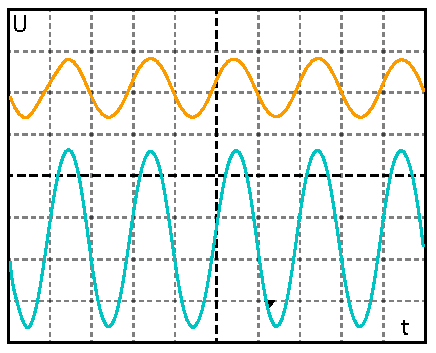
\includegraphics[width=0.7\linewidth]{4.jpg}}
    \caption{Перший плівковий накопичувач компанії IBM, IBM 726}
    \label{ris4}
  \end{figure}

Щоб домогтися такого прогресу, інженери пристосували головки для читання і запису рухатися по вкрай вузьких доріжках на плівці - близько 100 нанометрів шириною. Крім цього, довелося зробити зчитувальні головки вужчими - близько 50 нанометрів шириною. При зчитуванні рівень сигналу до шуму теж зменшився, тому довелося маніпулювати розміром і положенням намагнічених гранул і гладкістю поверхні плівки, а також удосконалити процес обробки сигналу і помилок зчитування.\par

Для того, щоб забезпечити надійність записаних даних протягом десятиліть, інженери розробили нові записуючі головки, що виробляють набагато сильніші магнітні поля, ніж звичайні.\par

Поєднавши всі ці розробки, інженерам IBM вдалося досягти щільності запису в 818000 бітів на лінійний дюйм (такий вимір щільності склався історично). Нова технологія дозволила вмістити на одному дюймі 246200 доріжок запису і надала місце для 201 гигабита на квадратний дюйм. Картридж з 1140 метрами плівки на котушці здатний зберегти 330 терабайт інформації. Це можна порівняти з цілою возом жорстких дисків.\par

Консорціум індустрії зберігання даних, куди входять HP, IBM, Oracle, Quantum\cite{lit2} і кілька дослідницьких груп, в 2015 році випустили документ про плани розвитку зберігання даних на плівці. За прогнозом консорціуму до 2025 року щільність запису на квадратний дюйм виросте до 91 гігабайти, а до 2028 року - до 200 гігабайтів.\par

Автори документа професійно зацікавлені в подібному оптимістичному прогнозі, але він цілком реалістичний. У лабораторії IBM підтверджують, що 200 гігібайтов на квадратний дюйм - здійсненне мета на найближче десятиліття.\par

Плівка - носій інформації, якого «закон Мура» притисне в останню чергу. Тому вигода від зберігання даних на плівці в порівнянні з жорсткими дисками буде збільшуватися в прийдешні роки.\par

Також відомо, що міжнародна група фізиків домоглася граничної щільності запису інформації в магнітному стані речовини - один біт в одному атомі. Це відповідає збільшенню ємності жорстких дисків в тисячі разів. Для двухбітового пристрою вчені розробили процедури запису та зчитування інформації за допомогою скануючого тунельного мікроскопа. Технологія ще далека від реальних застосувань, проте вона показує, що досягнення межі щільності запису інформації можливо. Дослідження опубліковане в Nature, коротко про нього повідомляє редакційна замітка журналу\cite{lit3}.\par

\begin{figure}[h]
  \center{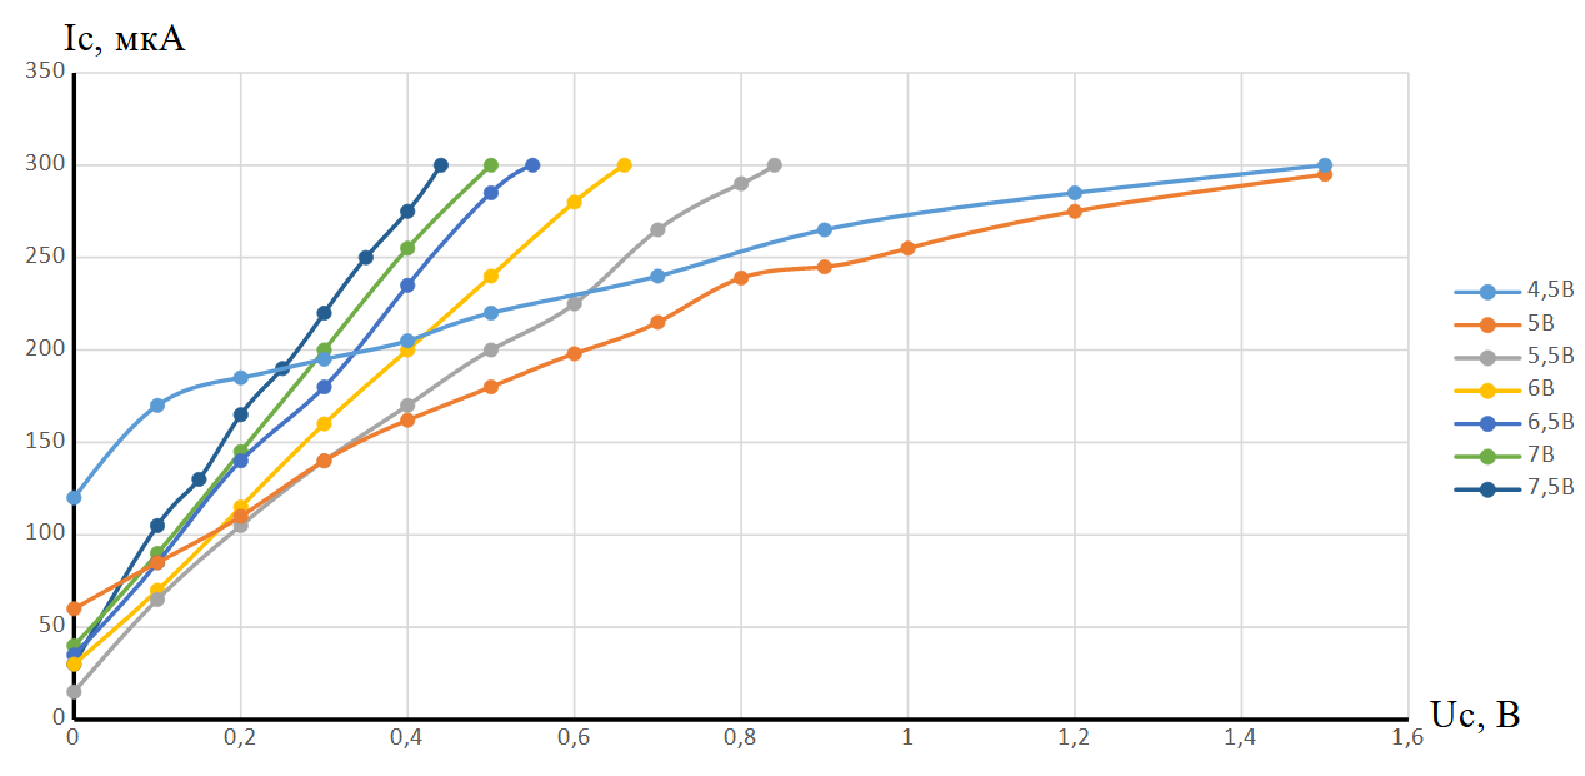
\includegraphics[width=0.9\linewidth]{5.jpg}}
  \caption{Мангітні біти в дискеті}
  \label{ris5}
\end{figure}

Як вже було описано раніше, магнітний запис інформації заснована на тому, що багато матеріалів в магнітному полі намагнічуються вздовж його ліній і зберігають цю намагніченість навіть після відключення поля. У магнітних носіях, таких як дискети і HDD, роль бітів виконує намагніченість невеликих ділянок диска. Зі зменшенням розмірів цих ділянок значно зростає обсяг інформації, яку можна записати на пристрої того ж розміру. Зараз один домен комерційно доступних жорстких дисків налічує в собі близько мільйона атомів (кілька нанометрів в діаметрі). Експерименти показують, що розмір комірки можна зменшити до 3-12 атомів.\par

Автори нової роботи домоглися стабільного запису і зберігання інформації протягом декількох годин в одиночних атомах гольмію. Вибір металу вчені пояснюють наступним чином. Будь-яка орбіталь атома може нести на собі жодного, один або два електрони. Магнітні властивості атомів визначаються в основному неспареними електронами, які знаходяться на своїй орбіталі на самоті. Гольмій володіє великою кількістю неспарених електронів і, до того ж, є володарем найбільшого магнітного моменту серед елементів періодичної таблиці. Крім того, неспарені електрони атома знаходяться близько до ядра, що забезпечує їх деяку ізольованість від зовнішнього середовища. Тому магнітний стан гольмію може зберігатися досить довгий час.\par

\begin{figure}[h]
  \center{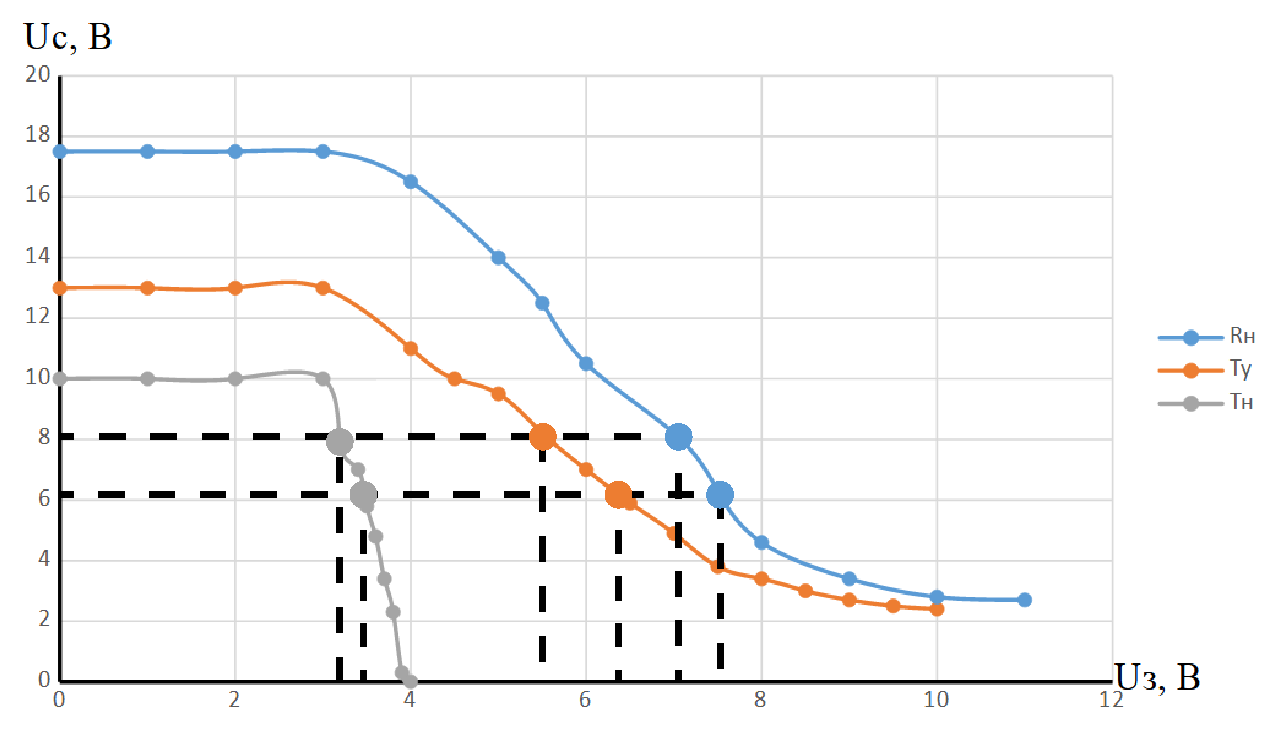
\includegraphics[width=0.9\linewidth]{6.jpg}}
  \caption{Схема експерименту (зліва). Читання станів атомів (праворуч).}
  \label{ris6}
\end{figure}


На поверхні оксиду магнію Гольмій відчуває магнітну анізотропію - вона призводить до того, що у атома є два стійких магнітних стана, що визначаються орієнтацією його сумарного спіна. Щоб перейти з одного стану в інший атом повинен подолати енергетичний бар'єр. Чим нижче температура середовища, тим менш імовірний цей перехід. Відповідно цим двох стійким станам і приписуються значення «нуля» і «одиниці».\par

В експерименті вчені створили комірку пам'яті, що складалася з двох атомів гольмію, що знаходяться на поверхні оксиду магнію, який був охолоджений до 1,2 Кельвіна. Для запису і читання вчені використовували скануючий тунельний мікроскоп, який досліджує поверхні за допомогою надзвичайно гострої голки. Операція запису полягала в додаванні до атому певної електричної напруги. Для читання автори використовували ефект тунельного магнітоопору - електричний опір між поверхнею і голкою залежить від напрямків намагніченості кінчика голки і атома гольмію. \par


\begin{figure}[h]
  \center{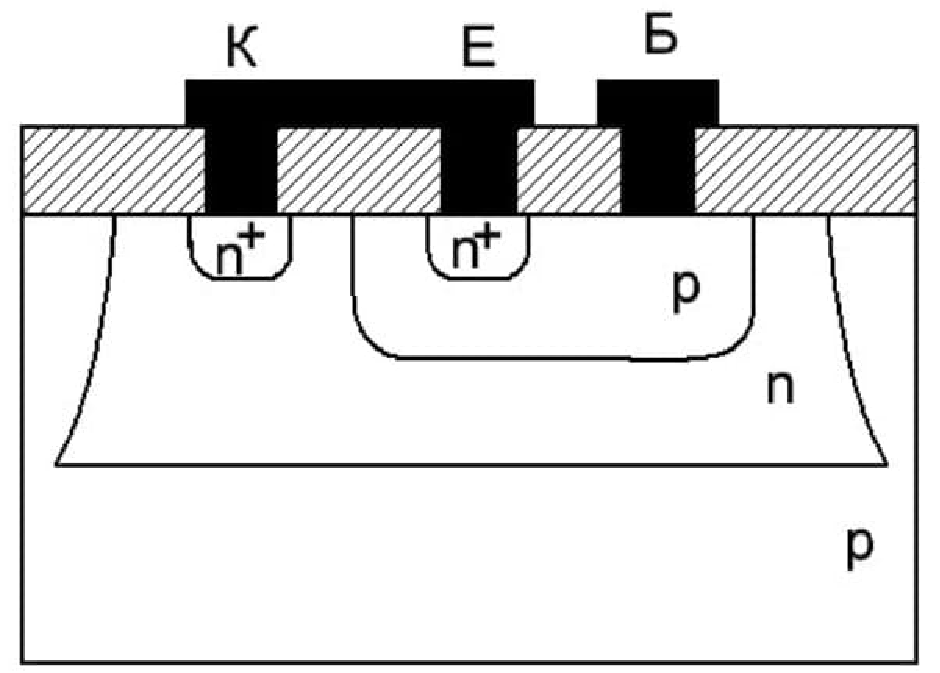
\includegraphics[width=0.7\linewidth]{7.jpg}}
  \caption{Спектроскопія атома заліза (праворуч) і біти - атоми гольмію (на скане зліва)}
  \label{ris7}
\end{figure}


Щоб перевірити, чи не вносить сама голка перешкод в роботу пристрою, і оцінити час життя записаної інформації, фізики використовували недавно розроблений ними метод моніторингу магнітних полів. Для цього поруч з атомами гольмію вчені помістили атом заліза, який служив детектором. Магнітне поле атома гольмію викликало невеликі зміни в електронній оболонці заліза (відбувалося розщеплення рівнів), що автори фіксували за допомогою спектроскопічних технік. Виявилося, що інформація зберігалася без змін на протязі більше п'яти годин. При підвищенні температури до 4,3 Кельвіна спонтанна зміна стану сталася через півтори години після запису.\par

Це не перший приклад пам'яті, що використовує для запису поодинокі атоми. У 2016 році голландські фізики навчилися кодувати інформацію за допомогою положення одиночних атомів хлору на монокристалі міді. Автори продемонстрували елемент пам'яті об'ємом в один кілобіт і навіть записали в нього фрагменти тексту лекції Річарда Фейнмана «Там внизу багато місця» і «Походження видів» Чарльза Дарвіна.\par

\begin{figure}[h]
  \center{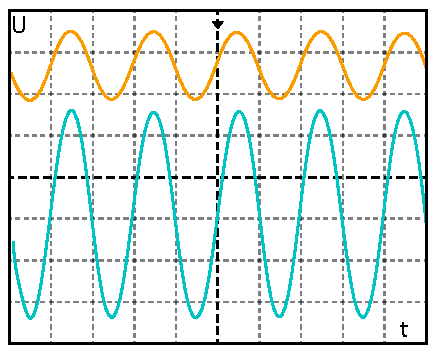
\includegraphics[width=0.9\linewidth]{8.png}}
  \caption{Зовнішній вигляд модуля пам'яті. Кожна клітинка - один атом}
  \label{ris8}
\end{figure}

Гранична щільність запису інформації дозволяє помістити по одному біту інформації в один атом, що знаходиться на поверхні носія. Якщо взяти, наприклад, поверхня монокристалла заліза і записувати інформацію на ній, то в квадратному сантиметрі вміститься близько 10 петабайт даних.\par

\begin{figure}[h]
  \center{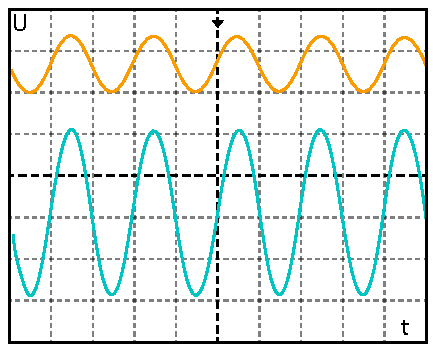
\includegraphics[width=14cm, height = 16cm]{9.png}}
  \caption{Текст, записаний в модулі пам'яті}
  \label{ris9}
\end{figure}



\begin{figure}[h!]
  \center{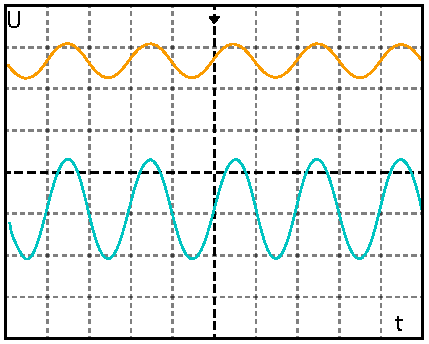
\includegraphics[width=15.5cm, height = 7cm]{10.png}}
  \caption{Принцип кодування інформації}
  \label{ris10}
\end{figure}

\clearpage
\newpage


Щільність запису в лабораторних зразках жорстких дисків, що використовують поздовжній магнітний запис, практично досягла теоретичної межі, і, хоча ця межа відсовуваляся неодноразово, більшість дослідників вважають, що в найближчі кілька років відбудеться перехід на іншу технологію запису. Як найбільш вірогідна це перпендикулярна технологія магнітного запису\cite{lit5} (рис. \ref{ris11}), що характеризується тим, що північний і південний полюси намагніченого ділянки розташовуються перпендикулярно поверхні магнітного диска. Такий напрям поля забезпечується конструкцією записуючої головки.\par

Перпендикулярний запис часто розглядалася як альтернатива поздовжнього запису\cite{lit6}, але в промислових масштабах перехід на неї був недоцільний, так як при щільності запису, з якими може працювати поздовжній запис, можливості цих технологій приблизно рівні, а вартість перпендикулярної технології трохи вище. Сьогодні перехід на технологію перпендикулярного запису обумовлюється тим, що її технологічні особливості дозволяють досягти більш високої щільності запису. При магнітному запису кожен біт утворює магнітний домен, що складається з певної кількості (зараз близько 100) магнітних зерен. Оскільки через особливості взаємодії двох сусідніх бітів при перпендикулярному записі оптимальна товщина робочого шару трохи більше, ніж при поздовжньої записи, необхідну кількість магнітних зерен займе меншу площу.\par

Більш ефективна геометрія магнітного поля, створюваного головкою, дозволяє збільшити щільність енергії магнітного поля в робочому шарі приблизно в чотири рази.\par

Крім того, різнойменні полюси намагнічених і ненамагнічених ділянок розташовані на протилежних сторонах робочого шару носія. Тому магнітні поля від сусідніх ненамагнічених ділянок будуть стабілізувати стан намагнічених ділянок. Це дозволяє помітно зменшити мінімальні розміри стабільних доменів.\par

\begin{figure}[h]
  \center{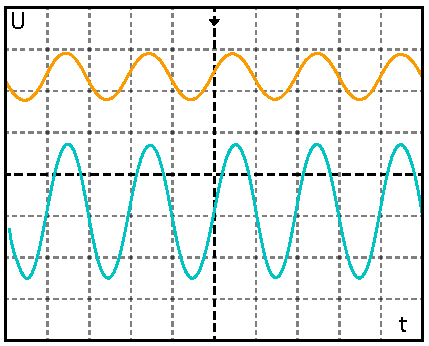
\includegraphics[width=0.7\linewidth]{11.png}}
  \caption{Принцип технології перпендикулярного магнітного запису}
  \label{ris11}
\end{figure}

За розрахунками фахівців компанії Seagate, перпендикулярний запис дозволить досягти щільності запису 1 Тбіт на 1 кв.дюйм, що еквівалентно можливості записати більше 1 Тбайт інформації на стандартний тридюймовий диск. Для наочності можна навести кілька цифр. Так, якщо роздрукувати 1 Гбайт текстової інформації з щільністю 2500 символів на сторінку, то висота стопки паперу складатиме близько 40 м. Для забезпечення щільності запису 1 Тбіт на 1 кв.дюйм необхідно досягти щільності розташування доріжок 500 тис. на 1 дюйм і лінійної щільності 2 млн. біт даних на 1 дюйм доріжки. При такій щільності на зрізі паперового листа вміщаються 2 тис. доріжок або 8 тис. біт даних.\par

Наведені цифри набагато перевищують ті, що можуть запропонувати сьогоднішні дискові накопичувачі, проте і цих показників щільності, беручи до уваги прогнозовані потреби в зберіганні даних в майбутньому, дуже скоро може виявитися недостатньо. Так, згідно з доповіддю Каліфорнійського університету в Берклі\cite{lit6}, щорічно в світі виробляється від 1 до 2 екзабайт (1 екзабайт еквівалентний мільярду гігабайт) інформації на найріхноманітніших носіях, включаючи магнітні, паперові, плівкові і оптичні. Не слід забувати і про те, що на магнітні носії поступово переводяться документи традиційного виду - паперові і плівкові, а крім того, зростають потреби побутової електроніки. Тому інженерам вже зараз доводиться шукати нові, ще більш перспективні технології запису і зберігання інформації.\par

В якості найбільш ймовірних кандидатів тут розглядаються термомагнітний запис HAMR\cite{lit8}  (Heat Assisted Magnetic Recording) і так звані самоорганізувальні магнітні решітки - SOMA\cite{lit7} (Self-Ordered Magnetic Arrays), однак на розробку цих технологій можуть піти ще роки.

Технологія термомагнитного запису схожа на технологію, використовувану в магнітооптичних приводах. При запису в обох випадках використовується залежність магнітних властивостей робочого шару від температури. Різниця між технологіями проявляється в способі зчитування інформації з диска. У магнітооптичних приводах інформація зчитується променем лазера, що працює на меншій, ніж при записі, потужності, а при термомагнитному записи інформація зчитується магнітної голівкою так само, як в звичайному жорсткому диску.\par

Запис інформації здійснюється шляхом нагрівання ділянки робочого шару, що знаходиться в магнітному полі записуючої головки. Нагрівання проводиться короткочасним впливом лазерного променя - тривалість імпульсу лазера менше тривалості магнітного імпульсу. Магнітне поле підбирається з таким розрахунком, щоб при відсутності нагрівання його величина була недостатньою для перемагнічування робочого шару. При підвищенні температури ділянки робочого шару відбувається суттєва зміна його магнітних властивостей: наприклад, може в 3-4 рази зменшуватися коерцитивної сили. Це призводить до того, що нагріті ділянки перемагнічуються. Подібні області і представляють собою записану інформацію.\par

Для термомагнитной записи використовуються матеріали з високою коерцитивної силою, що забезпечує високу стабільність записаних ділянок. Мінімальні розміри області, що відповідає одному біту інформації, визначаються діаметром сфокусованого світлового променя. За оцінками фахівців компанії Seagate, термомагнітна запис дозволить досягти щільності запису 10 Тбіт на 1 кв.дюйм.\par

В основі технології \href{https://compress.ru/article.aspx?id=10717&part=51ext1}{SOMA} лежить ідея створення невеликих ізольованих осередків магнітного матеріалу, організованих в регулярні масиви. На малюнку зображена фотографія масиву з щільністю запису 9 Тбит / кв.дюйм, отримана за допомогою електронного мікроскопа зі збільшенням 145 тис. разів, діаметр зерен(комірок) магнітного матеріалу менше 7 нм. Ось що каже з цього приводу один з її розробників, д-р Дітер Уеллер з Seagate Research: «\textit{Для запису одного біта інформації зараз необхідно приблизно 100 зерен магнітного матеріалу, ми ж працюємо над тим, щоб кожне зерно зберігало власний унікальний біт. Це дозволить різко збільшити щільність запису інформації. Ми шукаємо способи вибудувати магнітні зерна в правильні решітки, які не тільки дозволять зчитувати і записувати дані, але і забезпечать високу стійкість до температурних впливів}». Сьогодні вважається, що найкращим матеріалом для виготовлення таких носіїв є сплав заліза і платини з додаванням ретельно збалансованого співвідношення інших хімічних елементів.


Сучасні магнітні носії інформації, такі як HDD, мають фундаментальним обмеженням на межу щільності запису. Воно відповідає мінімальному розміру магнітного домена. Для того, щоб його обійти вчені шукають інші носії інформації. Наприклад, зберігати дані можна в ДНК - недавно в її молекулах \href{https://nplus1.ru/news/2016/07/07/200-mb-dna}{записали} близько 200 мегабайт даних. Але і в традиційних магнітних матеріалах ще є потенціал росту - \href{https://nplus1.ru/news/2016/05/19/six-state-memory}{використання} комірок, здатних перебувати в одному з шести, а не двох станів. Передбачається, що поєднання технологій SOMA і HAMR дозволить досягти щільності запису на магнітний диск 50 Тбіт на 1 кв.дюйм. На закінчення можна сказати, що в найближчі десять років розвиток технології магнітного зберігання даних має задовольнити зростаючі потреби ринку.\par







\begin{thebibliography}{9}
\bibitem{lit1} Основы магнитной записи информации : учеб. пособие для студентов физического факультета / сост. : С.П. Кудрявцева. – 2017. 51 с.
\bibitem{lit2} https://habr.com/ru/post/422851/
\bibitem{lit3} https://nplus1.ru/news/2017/03/09/information-density-record
\bibitem{lit4} II International Scientific Practical Conference of graduate and postgraduate students,
lecturers «APPLIED ISSUES OF EXACT SCIENCES»
19-20 October 2018, Armavir(http://amti.esrae.ru/pdf/2018/3(1)/197.pdf)
\bibitem{lit5} https://compress.ru/article.aspx?id=10717part=31ext1
\bibitem{lit6} https://compress.ru/article.aspx?id=10717
\bibitem{lit7} https://aip.scitation.org/doi/10.1063/1.1953879
\bibitem{lit8} \href{https://www.researchgate.net/publication/224354512_Heat_Assisted_Magnetic_Recording}{Heat Assisted Magnetic Recording}
\bibitem{lit9}  \href{https://essuir.sumdu.edu.ua/handle/123456789/80094}{Формування енергоефективних електронних інформаційних систем на основі феромагнітних композиційних матеріалів. Овруцький, М.С.2020}
\bibitem{lit10} https://essuir.sumdu.edu.ua/handle/123456789/80330
\end{thebibliography}
\end{document}
